\chapter{Copy Protection Status Quo}
\label{chapter:copy_protection_status_quo}

This chapter will first provide some detailed information about the ART runtime since the internal mechanics are a precondition to understand the more complex copy protection mechanisms and obfuscation techniques. The existing ones will be explained afterwards. Most of them are based on the Dalvik runtime. It will then be determined whether a specific method is also
applicable to ART. A great focus will of course rely on the DEX format since
it is still the distribution format of every app (inside of an APK).

\section{ART Internals}
\label{section:art_internals}

\subsection{APP Executable Format}\label{section:app_executable_format}

A core element of the recently introduced ART is the file that
gets created by ``dex2oat'' during the installation time of an app,
described in \autoref{section:app_installation}.
Since ART does use AOT compilation, the file format is expected
to be an executable or at least a native code container.
%A lot of copy protection mechanisms are based on the use of native
%code because it is supposed to be more secure from reverse code
%engineering (which is an assumption so far).
Therefore it's worth to have closer look at that file format
especially since Google does not provide any further information
about it's content and it might have the potential of
revolutionizing the available copy protection mechanisms for
Android or having at least a great impact on them.

By applying the Unix command ``\code{file}'' (which can classify
files to MIME-types) to the resulting file of the ``\code{dex2oat}''
tool it comes apparent that it's a particular ELF file (32 or 64 bit)
called OAT file from now on.

\subsubsection{ELF File Format}\label{section:elf_file_format}
ELF originally was originally specified by UNIX System Laboratories
(USL) and later by Tool Interface Standards (TIS) and is a common
standard for executables, object code and shared libraries on UNIX
systems. It's a quite flexible format for different CPUs and
architectures and does serve as a container for different
executable binary formats.

\begin{figure}[htb]
  \centering
  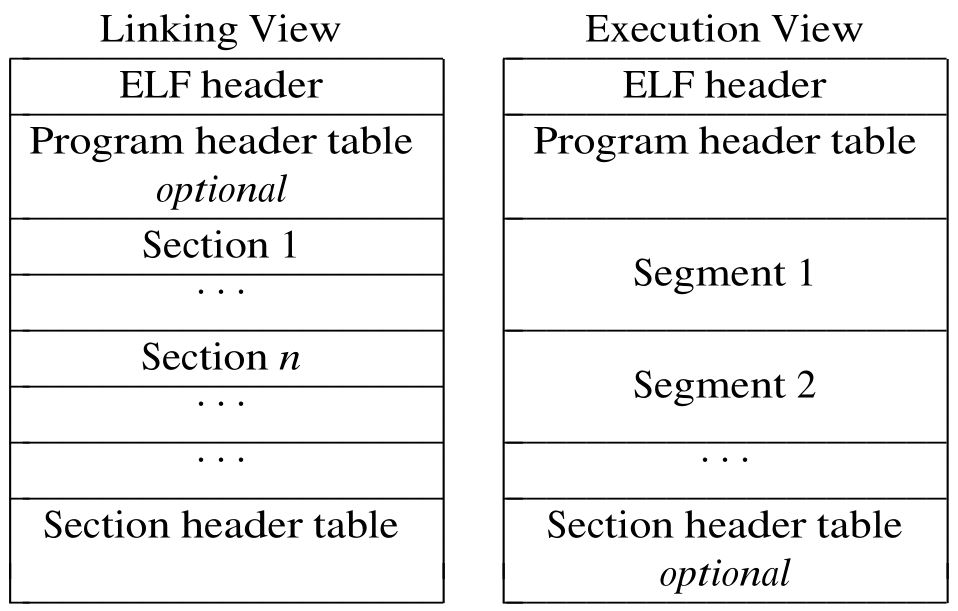
\includegraphics[scale=0.4]{figures/elf_format}
  \caption[ELF file format]{ELF file format taken from \parencite{portable_formats_spec}}
  \label{fig:elf_format}
\end{figure}

The \autoref{fig:elf_format} shows the file structure.
One have to differentiate the context of how the file is viewed.
While a linker does care about sections, sections may be
glued together to segments when executing the file.
Meta data about the file can be read out of the ``ELF header''
that starts at adress \code{0x00} and does contain
information about the version, file type, target machine and
offsets to the program- and section header tables.
In ART, the file is marked as an shared object with LSB encoding
and not as an executable which makes clear that this file is not
supposed to get executed directly but to be linked first
(An open question remains so far which process is then starting
the app).
Segments are referenced by the program header table and sections
by the section header table. For an execution process, only the header
and the information out of the program header table is needed
\parencite{life_of_binaries}.

Let's first have a look at the used sections in case of the specific
Android implementation, the OAT file:
\autoref{tab:section_headers} does show the output of
``\code{readelf -S <ELF-App-File>}'', listening all available sections


\begin{table}[htb]
  \caption[ELF section headers]{ELF section headers}
  \label{tab:section_headers}
  \centering
  \begin{tabular}{l l l l l l l l l l l}
    \toprule
    \multicolumn{11}{l}{Secion Headers:}\\
    \midrule
    {[}Nr{]} & Name & Type & Addr & Off & Size & ES & Flg & Lk & Inf & Al \\
    {[} 0{]} &      & NULL & 00000000 & 000000 & 000000 & 00 &    & 0 & 0 & 0 \\
    {[} 1{]} & .dynsym & DYNSYM & 000000d4 & 0000d4 & 000040 & 10 & A & 2 & 0 & 4 \\
    {[} 2{]} & .dynstr & STRTAB & 00000114 & 000114 & 000029 & 01 & A & 0 & 0 & 1 \\
    {[} 3{]} & .hash & HASH & 00000140 & 000140 & 000020 & 04 & A & 1 & 0 & 4 \\
    {[} 4{]} & .rodata & PROGBITS & 00001000 & 001000 & 002000 & 00 & A & 0 & 0 & 4096 \\
    {[} 5{]} & .text & PROGBITS & 00003000 & 003000 & 000228 & 00 & AX & 0 & 0 & 4096 \\
    {[} 6{]} & .dynamic & DYNAMIC & 00004000 & 004000 & 000038 & 08 & A & 1 & 0 & 4096 \\
    {[} 7{]} & .shstrtab & STRTAB & 00000000 & 004038 & 000038 & 01 &   & 0 & 0 & 1 \\
    \bottomrule
  \end{tabular}
\end{table}


It does follow a short description of sections that are implemented
\parencite{life_of_binaries}:
\begin{itemize}
    \item \code{.dynsym} holds a dynamic linking symbol table that
    does contain information for locating and relocating a program's
    symbol definitions and references. It does contain ``oatdata'',
    ``oatexec'' and ``oatlastword'' in case of an OAT file.
    \item \code{.dynstr} does hold strings for dynamic linking,
    mostly names that are referenced by \code{.dynsym}.
    \item \code{.hash} contains the symbol hash table
    \item \code{.rodata} stands for ``Read-Only data'' and does
    contain arbitrary data whose interpretation is solely
    determined by the program itself. We will
    see that in case of Android it does hold the actual OAT file
    that will be further described in \autoref{section:oat_file}.
    \item \code{.text} is the only region that is marked as
    executable and therefore it does hold the main body of
    program code.
    \item \code{.dynamic} includes dynamic linking information.
    \item \code{.shstrtab} stands for ``Section header string
    table'' and therefore contains the previous described
    section names including its own (e.g. ``\code{.shstrtab}'').
\end{itemize}

\autoref{tab:program_headers} shows the alternative view of the
file by having a look at segments (``\code{readelf -S <ELF-App-File>}'')
. Type ``PHDR'' stands for ``Program header''. Segments with type
``LOAD'' are supposed to be loaded from disk into memory while
a ``DYNAMIC'' segment is a part of a ``LOAD'' segment and is equal
to the ``\code{.dynamic}'' section. The mapping of ``LOAD'' segments
into memory is performed by respecting the alignment of \code{0x1000}
means that only chunks of that size (or a multiple) are being read
(e.g. reading the segment at \code{0x3000} will copy the content
from \code{0x3000-0x4000} even if the size only equals \code{0x340}).
The difference between ``FileSiz'' that obviously stands for the file
size and ``MemSiz'' that stands for memory size is the space that
gets reserved for uninitialized variables.

\begin{table}[htb]
  \caption[ELF program headers]{ELF program headers}
  \label{tab:program_headers}
  \centering
  \begin{tabular}{l l l l l l l l}
    \toprule
    \multicolumn{8}{l}{Program Headers:}\\
    \midrule
    Type & Offset & VirtAddr & PhysAddr & FileSiz & MemSiz & Flg & Align \\
    PHDR & 0x000034 & 0x00000034 & 0x00000034 & 0x000a0 & 0x000a0 & R & 0x4 \\
    LOAD & 0x000000 & 0x00000000 & 0x00000000 & 0x03000 & 0x03000 & R & 0x1000 \\
    LOAD & 0x003000 & 0x00003000 & 0x00003000 & 0x00340 & 0x00340 & R E & 0x1000 \\
    LOAD & 0x004000 & 0x00004000 & 0x00004000 & 0x00038 & 0x00038 & RW & 0x1000 \\
    DYNAMIC & 0x004000 & 0x00004000 & 0x00004000 & 0x00038 & 0x00038 & RW & 0x1000 \\
    \bottomrule
  \end{tabular}
\end{table}


The \code{readelf} tool is also capable of showing the resulting
mapping of sections to segments
(\autoref{tab:sections_segments_mapping}).


\begin{table}[htb]
  \caption[ELF section segment mapping]{ELF section segment mapping}
  \label{tab:sections_segments_mapping}
  \centering
  \begin{tabular}{l l l l l}
    \toprule
    \multicolumn{5}{l}{00}\\
    01 & .dynsym & .dynstr & .hash & .rodata \\
    02 & .text & & & \\
    03 & .dynamic & & & \\
    04 & .dynamic & & & \\
    \bottomrule
  \end{tabular}
\end{table}

It's interesting to note that the Android usage of ELF for apps
is very minimalistic and does contain very few sections/segments
compared to a common program written in C/C++ (\code{helloWorld.c}
does include over 30 sections). As described before,
\code{.dynsym} does contain entries which tell us where to find
the OAT data, specifically the ``oatdata''(equals \code{.rodata})
and the ``oatexec'' (equals \code{.text})
section that will now be analyzed.

\subsubsection{OAT File}\label{section:oat_file}
Google does not provide any official documentation about the OAT
file format other than the source code itself
(\code{art/runtime/oat[\_file].h[c]}). \parencite{hiding_behind_art}
however gives a helpful introduction and an overview is given
in \autoref{fig:oat_format} that shows the content of ``oatdata''.

\begin{figure}[htb]
  \centering
  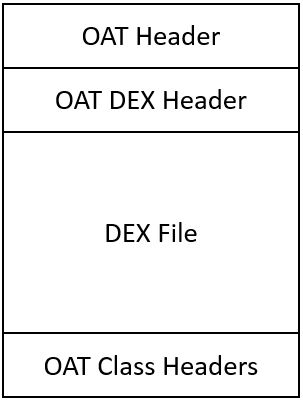
\includegraphics[scale=0.5]{figures/oat_format}
  \caption[OAT format]{OAT format}
  \label{fig:oat_format}
\end{figure}

Important attributes that the ``OAT Header'' contains are the
checksum over itself,
the instruction set (ARM, ARM64, MIPS, \ldots), the executable
offset (actually it is not standalone executable but just contains
native code instructions)
relative to the begin of ``oatdata'' and the quantity of embedded
DEX files (in case of apps it's always one, other system files like
``boot.oat'' may contain several DEX files). It does follow the
``OAT Dex Header'', containing
the absolute path of the ``source'' file (=DEX), the checksum, the
embedded DEX file's offset as well as
an offset to the ``OAT Class Headers''. ``OAT Class Headers''
do offer information about defined classes. It does include the type
of class, means how many methods in the class
are compiled to native code (``all'', ``some'' or ``none'' but
should be ``all'' in almost every case) and secondly
the offsets to the native code begin of every compiled method.
The actual code is located in a superordinated section
\code{.text} which is separated but referenced from this one.

\subsubsection{DEX File Format}
\label{section:dex_file_format}
To be complete, a description and explanation to the DEX format is also given,
which is officially documented by Google \parencite{dex}.
Before the introduction of ART, DEX was the last unit before
execution of an app (besides ODEX which can be easily converted back to DEX). The DVM does however accept
both formats and therefore it's possible to execute
DEX files without the transformation step. As a consequence,
DEX files can also be loaded dynamically at runtime which are not a part
of the distributed app. That enables new possibilities for dynamic code obfuscation techniques that will be described in \autoref{section:obfuscation_techniques}. DEX as it is does not only contain
VM instructions but some meta data around that to locate
higher abstraction level sections of the file like classes,
methods and fields.
\autoref{fig:dex_format} does show the file layout.
\begin{figure}[htb]
  \centering
  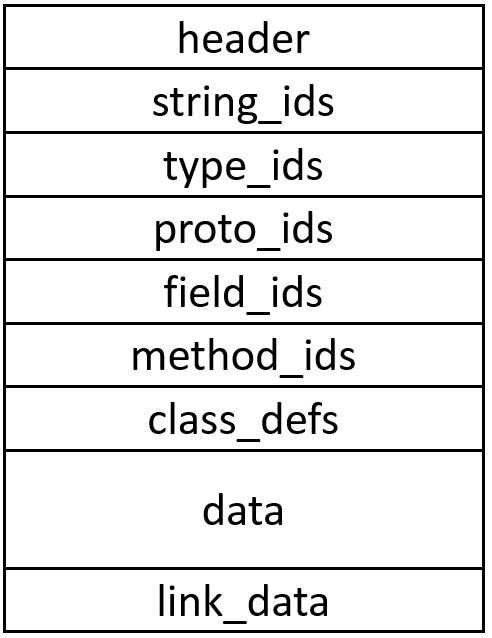
\includegraphics[scale=0.3]{figures/dex_format}
  \caption[DEX format]{DEX format}
  \label{fig:dex_format}
\end{figure}
The header again includes a checksum of the whole file (checksum
field excluded), the overall size as well as the offsets and sizes
of every section. Sections with ``ids'' ending are arrays of
id items of their type and do reference
a data item in the ``data'' section or are specifying
an index into another ``ids'' section. A ``string\_id'' item for
instance does just contain an offset from file beginning
that should be located in ``data'' whereas the ``type\_id'' item
includes an index into the ``string\_ids'' field. So every
attribute that can be described as a string is concentrated in ``string\_ids'' The principle of the file structure is therefore a architecture of referencing
sections. A part that puts everything together is the ``class\_defs''
section. Classes in this context stands for programming classes. They include methods which in turn include strings, fields and so on. Actual content like
strings, VM instructions or arbitrary programming data, is being stored exclusively in the data section. In the end, executable instructions are referenced from encoded methods, defined in ``class\_data\_items'' which in turn are referenced from ``class\_defs''.

%TODO: dex2oat nochmal gönnen!??

\subsubsection{Conclusion}\label{section:andelf_format_conclusion}
The runtime transition from DVM to ART of course had to result
in a new file that gets interpreted/executed when an app starts.
However, the change is not as smooth as expected since
the new file format is not pure executable code but, as
discovered, a combination of compiled native code
and embedded DEX code as well as a new OAT file format
which references parts of the native code. Also, there is some
confusion for what part the name ``OAT file'' stands. On the
one hand, Google's documentation files and the naming
convention of the``dex2oat'' tool are giving the impression
that the file as a whole is an ``OAT file''. On
the other hand, the file is a valid implementation of the
well known ELF format and contains a section that starts
with bytes known by MIME types with ``.oat'' as file format
(.rodata section). Additional, the ``oatexec'' section
is controlled via the greater ELF format. Therefore
, ``OAT file'' stands most likely for both of those meanings, the
Android app specific and minimalistic implementation of the ELF
as well as the combination of the ``oatdata'' and ``oatexec''
section to a file alike entity. \autoref{fig:andelf_format} does
provide an overall view of the file format of ART app executables.

\begin{figure}[htb]
  \centering
  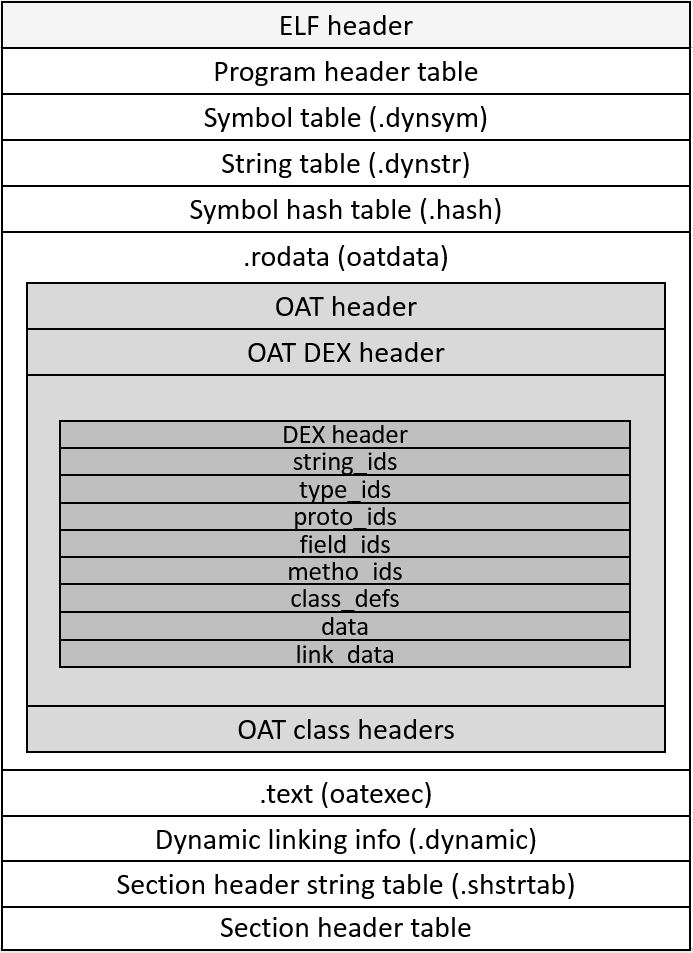
\includegraphics[scale=0.5]{figures/andelf_format}
  \caption[ART app executable format]{ART app executable format}
  \label{fig:andelf_format}
\end{figure}

The awareness of the detailed executable file format does pop
new questions about the ART internal functionality.
Since the file is marked as an shared object, it won't get
executed as a standalone program but most likely will be also
invoked in a forked Zygote process like in the Dalvik runtime.
However it is not clear which parts of the OAT file are
needed to run an app adequately. Is the embedded DEX for instance
mandatory for the app to work correctly? As it will be described
in a following chapter, DEX files are
a crucial part of applications to protect. What if that part
can be missed out by distributing a minimal stub application
followed by a dynamic native code injection at runtime?
It is also interesting if and how commong obfuscation
techniques designed for Dalvik, described in \autoref{section:obfuscation_techniques}, can be applied to ART.
Therefore a deep understanding for the app init and execution
process under ART is a precondition to answer those
questions and has to be more detailed than previously described in
\autoref{section:app_execution_simple}.

\subsection{App Execution}\label{section:app_execution_detail}
To get behind the scenes of the app execution, one can start at
the resulting Linux process that exists for every running app at
the end of the day.
The Linux tool ``\code{ps}'' can be used to display
running processes and therefore running apps.
To investigate the app execution a root shell at the target device
has to be opened (device should be rooted) with ``\code{adb shell}''
followed by an ``\code{su}'' command after getting the
device prompt (``\code{shell@flounder:/ \$}''), where \code{adb}
is the Android Debug Bridge to interact with connected devices.
The prompt will change to ``\code{root@flounder:/ \#}'' signaling
that it's a root shell. A ``\code{ps}'' command displays
process information like its owning ``USER'', the numerical process id ``PID'',
the process id of its parent ``PPID'' and of course the process name.
Interesting entries for further inspection are being displayed in
\autoref{tab:ps_entries}, showing the init, zygote, the chrome and
a sample hello world application.

\begin{table}[htb]
  \caption[Android Processes]{Android processes}
  \label{tab:ps_entries}
  \centering
  \begin{tabular}{l l l l l}
    \toprule
      USER & PID & PPID & ... & NAME \\
    \midrule
      root & 1 & 0 & ... & /init \\
      root & 211 & 1 & ... & zygote64 \\
      root & 212 & 1 & ... & zygote \\
      u0\_a137 & 10072 & 211 & ... & ma.schleemilch.helloandroid \\
      u0\_a35 & 11017 & 212 & ... & com.android.chrome \\
    \bottomrule
  \end{tabular}
\end{table}

The process ``\code{/init}'' is the first process of Android (although
it has a parent with PPID ``0'' but which is the process scheduler at kernel
level).
It can be derived that every user and system app has either the process
``\code{zygote}'' or ``\code{zygote64}'' as its parent process depending
if the app can be converted at the dexopt step to 32 or 64 bit.
That makes clear that apps are forked from the Zygote process which in turn
is a  fork of ``\code{/init}''.
Even more detailed information about processes can be
pulled out of the ``\code{/proc}'' directory (obviously an abbreviation for
``process'').
The directory offers an interface to the kernel space and does contain a folder for every process, named after its PID \parencite{proc}. The most attractive attribute for this investigation purpose of that folder is the
``\code{exe}'' attribute which is a symbolic link to the executable that started the process. Since apps are a fork of Zygote, they should also point
to the same executable, which they do (see \autoref{tab:process_executables}).

\begin{table}[htb]
  \caption[Process Executables]{Process starting executables}
  \label{tab:process_executables}
  \centering
  \begin{tabular}{l l}
    \toprule
    \multicolumn{2}{l}{root@flounder:/ \# ls -la /proc/10072/exe} \\
    ... & exe -> /system/bin/app\_process64\_original\\
    \midrule
    \multicolumn{2}{l}{root@flounder:/ \# ls -la /proc/211/exe} \\
    ... & exe -> /system/bin/app\_process64\_original\\
    \midrule
    \multicolumn{2}{l}{root@flounder:/ \# ls -la /proc/11017/exe} \\
    ... & exe -> /system/bin/app\_process32\\
    \midrule
    \multicolumn{2}{l}{root@flounder:/ \# ls -la /proc/212/exe} \\
    ... & exe -> /system/bin/app\_process32\\
    \bottomrule
  \end{tabular}
\end{table}

An executable named ``\code{app\_process32/64}'' seems like to be the entry-point for apps (or at least Zygote) to get started.
The responsible program of that executable
can be found in the Android Open Source Project (AOSP) where
``\code{app\_main.cpp}'' is the name of the source code file that gets
compiled into the 32 or 64 bit version
and can be found at ``\code{/frameworks/base/cmds/app\_process/}''.
Although its implementation allows apps to get started directly without
Zygote, they are not supposed to, means it's not the common way
when a user clicks on an app icon. Instead, it will get clear that Zygote
is capable of forking and specializing itself into a new app.
The app process is therefore responsible for starting Zygote and other system
related app like processes.
The ``\code{/init}'' process arranges the start of Zygote via an
``\code{app\_process}'' program start with specific parameters for a Zygote start
(init is responsible for far more, like starting native daemons system services and other things).

A comman way to analyze source code is to start at its
``\code{main()}'' method.
One of the first things the program does is
creating a new ``\code{AppRuntime runtime}'' object that inherits from the
\code{AndroidRuntime} class but does override a few functions. As parameters it will expect the \code{argv[0]}
which is the program name itself as well as the total length of arguments.
Finally, the program will transfer the flow control to this object by calling
\code{runtime.start(com.android.internal.os.ZygoteInit, args)} in case of a
Zygote start.
``\code{args}'' contains whether to start the system server and an ABI
list as well as remaining arguments that were not used for the \code{app\_process} program. The runtime \code{start()} method does initialize
a VM and finally calls the main method of the \code{ZygoteInit.java}
program in case of a Zygote start. So there is a first transition into the Java programmed system.

\subsubsection{Zygote}\label{section:zygote}
\code{ZygoteInit's} main starts with parsing arguments such as if a system
server should get started, the ABI list and the socket name that Zygote will
create. That defined socket (\code{LocalServerSocket sServerSocket}) is a core functionality of Zygote whose purpose
is to listen on a socket for app start requests and finally fork Zygote and specialize it afterwards. After registering that socket a preloaded method loads classes
resources, OpenGL and shared libraries and a explicit garbage collection
\code{gc()} will be performed to clean up after startup. After the optional start of the system server, the program will enter its main loop
\code{runSelectLoop(abiList)}. Garbage collection gets explicitly called
after \code{GC\_LOOP\_COUNT} iterations. Right before the loop an array list for file descriptors (\code{ArrayList<FileDescriptor> fds}) as well as for socket connections (\code{ArrayList<ZyogteConnection> peers}) is being
created and \code{fds} gets filled with the server socket file descriptor.
\autoref{zygote_init_loop} displays the logic of the main loop.

\lstinputlisting[language=Java, caption=ZygoteInit main loop, label=zygote_init_loop,firstline=773, lastline=795]{"code/ZygoteInit.java"}

First the file descriptor list is converted to an array and index gets
filled with a readable file descriptor. If that index is zero,
a new \code{ZygoteConnection} is established which is listening
on its defined socket and accepting pending connections.
Afterwards, it gets added to the \code{peer}
and \code{fds} list.
The \code{acceptComandPeer()} method does
call the \code{ZygoteConnection} constructor with \code{sServerSocket.accept()}
as transfer parameter which is an extension to the \code{LocalSocket}
implementation. Its \code{accept()} method accepts a new connection
to the socket and blocks until a new socket arrives.
Therefore the next iteration delivers an index greater than zero so that
the last \code{else} branch of \autoref{zygote_init_loop} is executed within
a \code{ZygoteConnection} object of \code{peers} at that index calls
the \code{runOnce()} method and gets removed out of the array lists afterwards.
Finally the \code{runOnce()} method will call \code{Zygote.forkAndSpecialize()}
that forks a child within an exception is being called to invoke the child's
\code{main()}.
But first the given arguments from the command socket must be parsed with the
aid of an \code{Arguments} class. Attributes that are needed for the later \code{fork()} call are shown in \autoref{tab:argument_class_attributes}.

\begin{table}[htb]
  \caption[Arguments Class Attributes]{Arguments Class Attributes}
  \label{tab:argument_class_attributes}
  \centering
  \begin{tabular}{l l l}
    \toprule
     Given Argument & Attribute & Description \\
     \midrule
     -{}-setuid & int uid & UNIX uid for the child \\
     -{}-setgid & int gid & UNIX gid for the child \\
     -{}-setgroups & int gids[] & additional groups \\
     -{}-enable-debugger & int debugFlags & debug information \\
     -{}-enable-checkjni & int debugFlags & debug information \\
     -{}-enable-assert & int debugFlags & debug information \\
     -{}-enable-safemode & int debugFlags & debug information \\
     -{}-enable-jni-logging & int debugFlags & debug information \\
     -{}-mount-external & int mountExternal & storage to mount \\
     -{}-target-sdk-version & int targetSdkVersion & target version \\
     -{}-classpath & String classpath & absolute classpath \\
     -{}-runtime-init & boolean runtimeInit & new runtime init \\
     -{}-nice-name & String niceName & process renaming \\
     -{}-instruction-set & String instructionSet & instruction set to use \\
     -{}-seinfo & String seInfo & SELinux infos  \\
     -{}-rlimit & ArrayList<int[]> rlimits & resource limitations \\
     -{}-app-data-dir & String appDataDir & data directory \\
      \bottomrule
  \end{tabular}
\end{table}

Then all the defined security policies are being applied. To avoid bad file
descriptor messages after forking a child, a native code has to close them before (\code{sServerSocket} and the local socket \code{mSocket} of the
\code{ZygoteConnection} class whose FDs are written into an \code{fdsToClose}
array).
Now all prerequisites of forking are fulfilled and the static method
\code{forkAndSpecialize} of the \code{Zygote.java} file can be called
(see \autoref{zygote_fork}) returning the new process PID.
\begin{lstlisting}[language=Java, caption=Zygote Fork Call, label=zygote_fork]
pid = Zygote.forkAndSpecialize(parsedArgs.uid, parsedArgs.gid,
            parsedArgs.gids, parsedArgs.debugFlags, rlimits,
            parsedArgs.mountExternal, parsedArgs.seInfo,
            parsedArgs.niceName, fdsToClose,
            parsedArgs.instructionSet,
            parsedArgs.appDataDir);
\end{lstlisting}
\code{Zygote.java} is quite compact since it mainly defines the transition
to native code where the actual forking is being applied on linux level. That's why
a native version of the fork and specialize method is defined and executed
which in turn returns the resulting PID after forking
(\code{com\_android\_internal\_os\_Zygote.cpp}).
The native implementation does finally call the effective \code{fork()} method
that copies the actual Linux process. Afterwards, the child is being
specialized (selected by the resulting PID of \code{fork()}).
Transfered FDs get closed and capability boundaries are applied.
UID and GID are being set (Linux \code{setresgid/setresuid}) and resource limits are added via \code{strlimit(2)}.
If necessary, a native bridge will be initialized and scheduler policies
are being set. SELinux properties are applied and the thread name gets
changed to a name other than ``app\_process'', mostly the package name of the app.

Back in the Java world \code{Zygote\allowbreak Connection} checks the returned PID and either calls \code{handleChildProc()} in case of the child or
\code{handleParentProc()} in case of the parent (Zygote itself).
These methods are handling the post fork setup. In case of the child, sockets are being closed on Java level (since the child should not listen on sockets like the parent Zygote) and remaining arguments are being evaluated. When forking an app, a class name will be defined at that time. Remaining arguments are copied to \code{mainArgs} and a class loader (\code{ClassLoader cloader}) is being defined before calling \code{invokeStaticMain()} of \code{ZygoteInit} with \code{cloader}, \code{className} and \code{mainArgs} as parameters. The class loader \code{cloader} is defined as
either with \code{PathClassLoader()} or \code{ClassLoader()} constructor whether a classpath is
given (path to APK or raw *.dex) where \code{PathClassLoader} is a specialized version of \code{ClassLoader}.
However when looking into the class loading code at this point, it becomes clear that the DEX file of an app is used to represent a class and later finding its main method within, so that
it can be said for sure that an app's DEX file is needed at least as an entry point under ART.

The \code{invokeStaticMain()} loads the specified class via the \code{className} string and furthermore searches for the main method within, storing it as a Java \code{Method} object and finally throwing an
\code{MethodAnd\allowbreak ArgsCaller()} exception. This exception gets caught by the main method of \code{Zygote\allowbreak Init}.
Remember that the Zygote itself is ``trapped'' in a loop whereas the child process can escape from by throwing that exception. So as a result, Zygote will remain in the loop offering a socket to fork itself again (=starting a new app) while the child process (=the app to start) escapes from that loop invoking the main method of the class specified over the socket
connection in the next step.
To clarify the program flow, \autoref{fig:zygote_forking} displays
the object and therefore file interaction during the forking process.

\begin{figure}[htb]
  \centering
  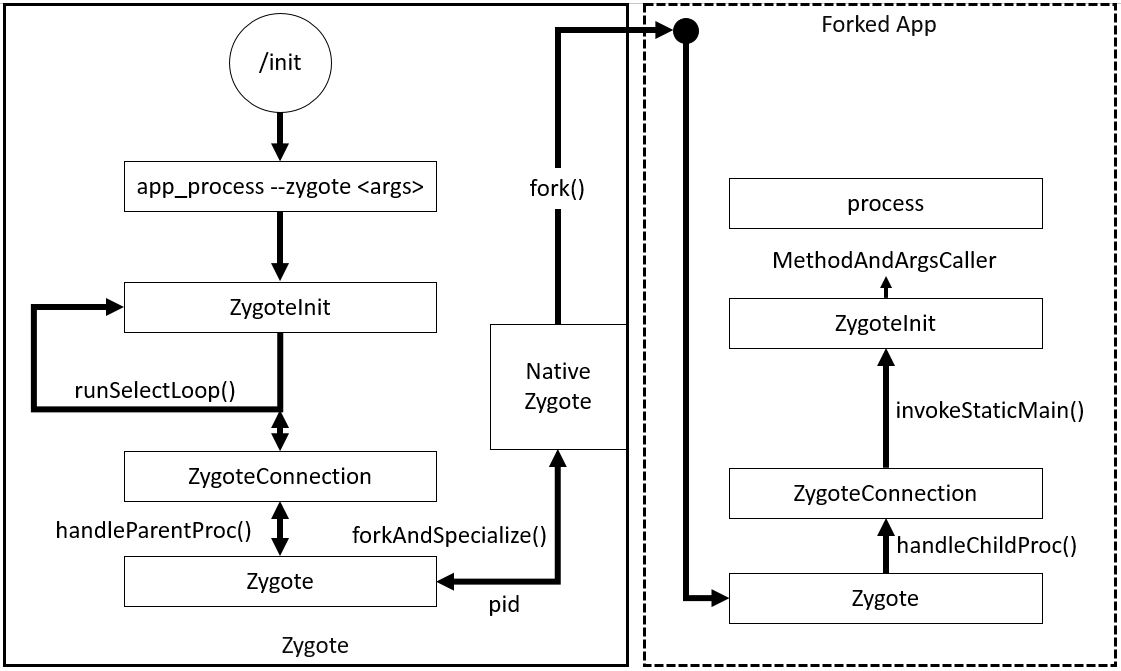
\includegraphics[width={\textwidth}]{figures/zygote_forking}
  \caption[Zygote Forking]{Zygote Forking}
  \label{fig:zygote_forking}
\end{figure}


The current child process state discussed is right after the main loop
breakout of \code{ZygoteInit} induced by the exception. The exception
is actual defined as a class that extends \code{Exception} and implements
\code{Runnable}. Therefore it is viable to call the exception callers
\code{run()} method (see \autoref{child_breakout}, taken out of the main
method of Zygote).

\lstinputlisting[language=Java, caption=Zygote Child Loop Breakout Exception, label=child_breakout,firstline=697, lastline=703]{"code/ZygoteInit.java"}


\subsubsection{Method Invocation}\label{cl_loading}
Invocation means basically injecting the code of a method in the current process.
In case of Android there exists the Java world as well as the Linux/native world.
Zygote does exist in both worlds (Java: \code{Zygote.java, ZygoteConnection.java, \ldots}
and native: \code{app\_process call with -{}-zygote}). The runtime is responsible for
executing Java layered code.

\code{ZygoteConnection} creates the \code{ClassLoader} instance and commits it to
\code{ZygoteInit} via the \code{invoke\allowbreak Static\allowbreak Main()} method. If the class specified
in \code{className} can be loaded successfully, the class loader tries to initialize a
\code{Method} instance of the defined classes main method.
That instance \code{m} gets finally transfered to the explained exception that gets thrown
at this point and finally the method instance \code{m} does call
\code{invoke(null, new Object[] {mArgs})} where \code{mArgs} represents a string array of
arguments. That method is defined in the official Java Documentation \parencite{java_method} since \code{m} represents the common \code{Method} class but is adapted for Android's needs.

This is where it gets interesting. The most recent state of the app starting process
right now is the forked and adapted process to the specific application. Now, the actual main
method gets invoked and later executed. Therefore the next step will reveal how ART will handle the created OAT files for apps with embedded dex and native code with its structure explained in \autoref{section:app_executable_format}. The invoke method in the \code{Method} class dis implemented as native code, means C++ (see \autoref{method_invoke}).
\lstinputlisting[language=Java, caption=Method Invoke Native Signature, label=method_invoke,firstline=370, lastline=376]{"code/Method.java"}
The \code{receiver} parameter represents the object the method gets called on. Therefore
in case of a static main method, it is \code{null}. The native implementation of \code{invoke}
is quite short and forwards the call to \code{InvokeMethod()} located in
``\code{reflection.cc}''. Those files are located at ``\code{/art/runtime/native}''.


After the size of the stack has been checked, an \code{ArtMethod* m} pointer gets initialized with its Java method (\code{Method} class) and through ``\code{art\_method.cc}''s static \code{FromReflecetdMethod()}. It does follow a few checks about the receiver (if \code{m} is static or
not)

TODO: To be finished or cutted if not getting into further Detail!

%When a user clicks on an app icon, the ``onClick()'' method
%of the ``Launcher'' application gets called.


\section{DEX Disassembly and Repackaging}
Like introduced in \autoref{chapter:android_status_quo} there
are different goals of copy protection mechanisms starting from
preventing reverse code engineering to protect intellectual property
and reaching to hinder patching to get prohibited access.
The common denominator of those goals is the protection of
the DEX file of every app since every distributed app does include
it. A variety of tools do exist that
are able to transform DEX into different readable formats,
modify it and repack it again since the DEX contains
a lot of meta data for its contents (classes, methods, \ldots)
\parencite{dex}.
Generally there do exist two possible outcomes of DEX disassembling
- Java code (\code{*.java}) and Smali code (\code{*.smali}).
Since the DEX format is more or less just a different mapping of a
JAR and its containing \code{.class} files, the transition to JAR
is quite simple \parencite{dvminternals}. A tool that is able to
perform this step is ``dex2jar'' \parencite{dex2jartool}.
Along with this JAR, standard Java decompilers like ``JD-GUI''
\parencite{jdtool} can be used to produce the \code{*.java} source code.
If the \code{*.java} is supposed to change and repacked, it can
again be compiled into JAR with Oracle's ``javac'' \parencite{javactool}
followed by Google's ``dx'' tool \parencite{dxtool}
to produce the new manipulated DEX.

An alternative way is the use of the ``smali/baksmali'' tool
\parencite{smalitool} which is a direct assembler and disassembler
for DEX files rather than taking the Java code detour. There is also
a tool included that can convert the ODEX back to DEX (which was interesting
for Dalvik Runtime systems).

Overall, the disassembly of unchanged DEX is quite easy and is shown
as a concluding overview in \autoref{fig:dex_disassembly}

Therefore several countermeasures were established which are
described in the following sections.

\begin{figure}[htb]
  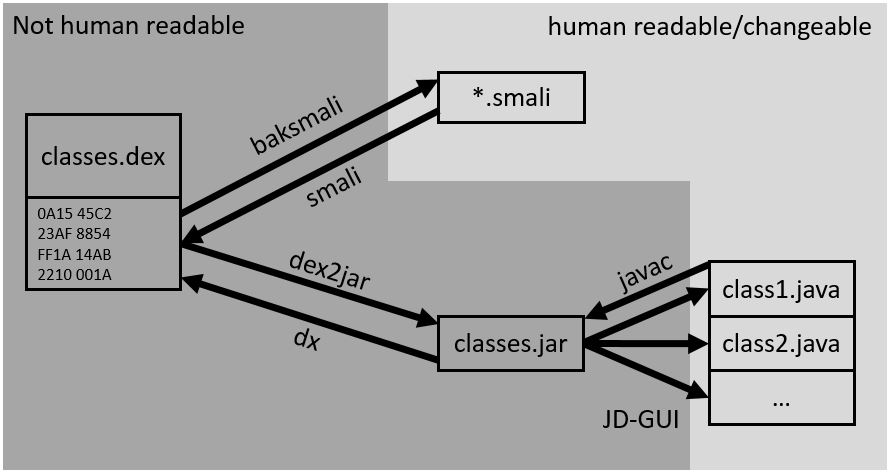
\includegraphics[width=\textwidth]{figures/dex_disassembly}
  \caption[DEX Assembly/Disassembly]{DEX Assembly/Disassembly}
  \label{fig:dex_disassembly}
\end{figure}


\section{Obfuscation Techniques}\label{section:obfuscation_techniques}
Obfuscation in the context of copy protection for application
is generally the term for hardening an application against
reverse code engineering techniques. It can be achieved by different methods
that can be separated in two main groups, static and dynamic obfuscation.
Static means that the obfuscation technique is applied to code units (source
code, binaries, ...) while the application is not executed. Therefore an
attacker could possibly successful analyze the application without executing it
if he manages to break this obfuscation. An upside of static techniques in general is that they are independent of the following runtime if two compared runtimes are using the same input files (which they do in case of Android, DEX).
Applications that are dynamically obfuscated on the other hand, are much harder to analyze. The behavior
of the application is not decided until its execution. An attacker needs to connect to the process of the running application followed by a just in time inspection. Dynamical methods do have the downside that they are highly dependent on the runtime.

It does follow a list of common static and dynamic obfuscation techniques
for Android applications. However, this list is mainly focused on
the Dalvik runtime since ART has been released quite recently.
Where static obfuscation techniques do show the same behavior in both
runtimes, the dynamic solutions do possibly not since the execution process
of apps in ART differs (described in \autoref{section:app_execution_detail}).
The impact of those techniques to ART will get analyzed at every specific case.


\subsection{Static}
\subsubsection{Common Source Code Obfuscation}
The most common and simple way of harden source code is to remove any kind of meta data
that has been added during the development process. Means destroying/modifying
information that originally was present in the source code.
Possible prospects to do this are the renaming of string identifiers of
classes, variables, methods and functions, to artificially insert
irreducible code, create artificial parallelization, perform method inlining/outlining, to unroll loops, encoding strings or changing the control flow in
order to confuse code analysts by keeping the original behavior
\parencite[p.87]{lvl_imp}.

Popular tools for that purpose are Google's ``ProGuard''
\parencite{proguardtool} which is included in the Android build system and
can be enabled easily as well as``DexGuard'' by GuardSquare
\parencite{dexguardtool}. ``ProGuard'' does
operate on source code level where ``DexGuard'' operates on DEX.
Since the first ``layer'' of Android applications is Java code, classical Java
obfuscators also can be used.
Since those tools do operate on the DEX file layer, they can be applied at ART without restrictions.

\subsubsection{Junk-Byte-Insertion}
Junk-Byte-Insertion's goal is to prohibit the use of program analyzing
disassembling tools. It does work for tools using the
``linear sweep'' method to analyze a program. That means
the tools are processing every instruction from the entry-point
till the end without interpreting them (e.g. not following jumps).
That examining technique can be exploited to break the disassembling
procedure. Let's assume we do have the following DVM instructions (Example taken out of \parencite[p.67]{lvl_imp}).
\autoref{junk_byte_listening}
  \begin{lstlisting}[language={[x64]Assembler}, caption=Junk-Byte-Insertion, label=junk_byte_listening, numbers=left]
    if "true" goto line 4
    load_array_into v1, line_3
    array_size 10
    set v2, 1
    set v3, 1
    add v1, v2, v4
    return v4
  \end{lstlisting}

Because of the if statement that performs a jump to line four, the \code{array\_size 10} command will never be reached.
Since ``linear sweep'' does not perform jumps, the analyzing tool
will interpret the ten following bytes of that array initialization as payload and will therefore not be able to disassemble the actual instructions.

Enhanced tools will use the ``recursive traversal'' technique to analyze a
program which is capable of detecting dead branches and conditional jumps like in the example above.
These tools also may be tricked by choosing a more complicated condition for
if-conditions that can only be evaluated at runtime and therefore the
whole conditional branch (including the breaking byte sequence) would also tried to be evaluated (Actually this technique could already be counted to dynamic obfuscation) \parencite[p.68]{lvl_imp}.


This example is based on DVM instructions and was therefore designed for Dalvik and
Android prior version five. 
The Junk-Byte Insertion will no more be possible in ART. Why? 
Even if one would insert Junk-Bytes into the DEX file, there is still a conversion
step into the new OAT format introduced in ART, which compiles into native code so 
that any form of inserted bytes wont be adopted. So Junk-Bytes can of course still
be inserted into DEX to prevent an attacker to perform disassembling of DEX but those
Junk-Bytes will not apply to the compiled code. However, since the compiled code
is native code and therefore not that easy to disassemble, Junk-Bytes might still be
usefull at DEX layer.

\subsection{Dynamic}
\subsubsection{Hidden Methods Invocation}
In \parencite[p.82f]{lvl_imp} a technique is described to hide a whole method
in \code{.dex} files. This hiding method is highly dependent on the DEX specification from Google \parencite{dex} that has been described in
\autoref{section:dex_file_format}.
It does base on the fact that the actual instructions of methods residing
in the \code{data} section of a DEX are referenced but not parsed directly
by sweeping over that file area so that the metadata section of methods
includes an offset to its actual instructions.
These references (which are offsets into the data section) can be manipulated
to hide specific methods when the DEX gets parsed. Like shown in
 \autoref{fig:hidden_method_invocation} one could manipulate
 an offset pointer (in this example the offset from method one)
to hide its implementation.
In order to achieve this effect, a few bytes obviously need to be changed
(the offset value).
Since the DEX format includes a checksum to be resistant
against transmission errors, a revaluation is necessary.
After that hiding step, the method is invisible for static analyzing tools
but of course also for the DVM itself, means it is no more runnable.
Thats why the changes to the DEX need to be reversed at runtime.

\begin{figure}[htb]
  \centering
  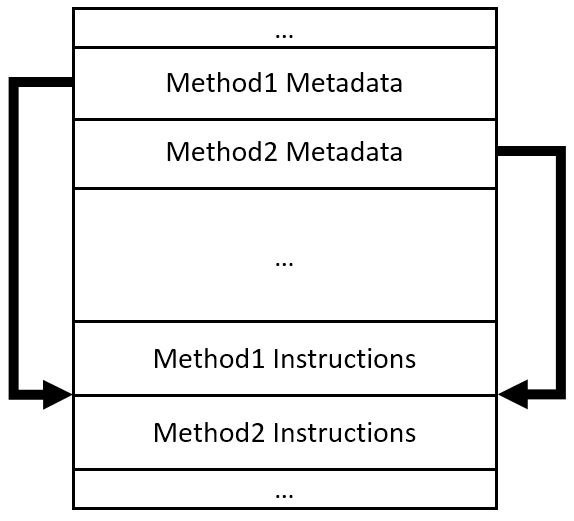
\includegraphics[scale=0.4]{figures/hidden_method_invocation}
  \caption[Hidden Methods Invocation]{Hidden Methods Invocation Principle (Method1 gets hidden)}
  \label{fig:hidden_method_invocation}
\end{figure}

A precondition for the Hidden Methods Invocation technique is the
possibility to load DEX files dynamically at runtime in order to revert
those changes. Otherwise a manipulation of the DVM bytes in a running app in RAM would be necessary to revert them. The next section deals with dynamic
code loading in general and will therefore cover the feasibility for Dalvik
and ART.

\subsubsection{Dynamic Code Loading}\label{section:dynamic_code_loading}
The principle of Dynamic Code Loading is to reveal the actual program code
not before running the application. This behavior can be achieved by
implementing a stub code that will then load the actual application
followed by execution. The format of that distributed application is
obviously the DEX, at least in Dalvik. If DEX still can be used
for ART has to be determined. In \parencite{dexfileclass} a practical
sample implementation for Dalvik is given.
To provide a copy protection benefit, an additional application file can either be distributed encrypted within the app stored in the \code{assets} folder or it can be fetched from a server.
Android does provide a public method within
the \code{DexFile} class to dynamically load DEX files
(\code{loadDex(String sourceName, String outputName, int flags)})
and loading included classes. The \code{sourceName} parameter accepts
a path to a JAR or an APK and \code{outputPathName} specifies
the file in which the optimized DEX version will get saved (ODEX in Dalvik).
That behavior however is a problem because the created ODEX will persist
also after closing the app and therefore can be analyzed after a one time
execution. Unfortunately it also can't be deleted cause of missing permissions.
In \parencite{code_protection},
a circumvention to that problem is described by using the JNI.
The \code{libdvm.so} library does offer a private method to open DEX files
that does accept DEX content in form of a byte array.
By establishing this own JNI implementation of
\code{openDexFile(byte[]content)} the loaded dex file is only present
in volatile memory and does not create an ODEX \parencite{code_protection}
which does make that method very robust. So the big question here is if
that method also can be applied to ART since \code{libdvm} has been replaced
with \code{libart}.

First it will be tried to load a DEX in ART with given Java APIs.
Like mentioned, \code{loadDex()} is a possible method but should be called
through a \code{DexClassLoader()}. It does expect a \code{dexPath} String where to look for Dex files, an \code{optimizedDirectory} String specifying a path to store the optimized version as well as a \code{parent} ClassLoader.
Like mentioned, the Dex to load can be shipped within the assets folder.
So at first a Dex is needed. For simplicity reasons a simple Java class will be used, showed in \autoref{java_class_to_load}.
\begin{lstlisting}[language=Java, caption=Java Class to load, label=java_class_to_load, numbers=left]
public class ToLoad{
    public int exampleMulMethod(int a, int b){
        return a * b;
    }
}
\end{lstlisting}
A Dex can be created with a ``\code{javac ToLoad.java}'' call followed by
using the \code{dx} tool with ``\code{dx -{}-dex -{}-output="toload.dex"
ToLoad.class}'' (Be sure to use a Java version < 1.8, otherwise the \code{dx}
command will fail since Java 1.8 ist not yet officially supported by Android at the time
of writing this thesis).
The \code{dexPath} has to be readable by the app itself. Therefore
the Dex should be stored in the app data directory where dexPath should then
search for, same for the optimized directory.
\code{getDir()} can create a private folder with a given name
and privileges. With \code{getAssets().open()}, the Dex can be
copied out of assets to the new data location by using buffered Java streams (see \autoref{dex_internal_storage}).
\lstinputlisting[language=Java, caption=Dex Internal Storage, label=dex_internal_storage,firstline=27, lastline=41]{"code/DexLoading.java"}
Now the \code{DexClassLoader()} constructor can be called with the recently
created paths and the context class loader. After that, the class can be loaded
by its name as well as getting the method with defining its argument classes.
Finally, \code{invoke()} can be called with a reference of the object to call
on (\code{null} if method is static, \code{newInstance()} if not) and its
arguments (\autoref{dex_method_invocation}).
\lstinputlisting[language=Java, caption=Dex Method Invocation, label=dex_method_invocation,firstline=45, lastline=54]{"code/DexLoading.java"}
The optimized output file is given in OAT format.
So the dynamic DEX loading is generally possible in ART with purely official
Android Java methods. However, the execution of code loaded that way should
be very slow since the Dex file gets optimized in an ART way (=compilation
into native code) and it doesn't really fit into the ART AOT compilation
philosophy. With that in mind, it should be clear that it is not possible
to load a Dex file into a byte array and execute it directly like it was
possible at Dalvik using the libdvm library via JNI since ART cannot execute
DVM instructions by design. So in the scope of copy protection mechanisms
with ART, dynamic code loading at Java layer is not that useful anymore. 
Instead it needs to get analyzed how code can be loaded dynamically in ART which 
will be determined in \autoref{chapter:android_dynamic_native_code}.

\subsubsection{Self Modifying Code}
Quite similar to dynamic code loading described in
\autoref{section:dynamic_code_loading} is self modifying code with the goal
of altering the instructions of an app during runtime.
Instead of loading additional code snippets, the focus relies on
manipulating the executing Dalvik byte code stream directly.
The DVM is limited in terms of instructions for modifying byte code
and therefore it has to be bypassed with native code via the JNI.
To find the position in byte code that should be changed, a predefined
value must be set in order to be recognized by the native code function.
That value is often called ``egg'' and the search process ``egg-hunting''.
Let's assume we do have the code snippet shown in \autoref{self_modifying_code} that exists in the context of an Android app activity
\parencite{code_protection}.
 \begin{lstlisting}[language=Java, caption=Self Modifying Code Example, label=self_modifying_code]
    ...
    modifyVariable();
    int egg = 0x12345678;
    Integer toChange = 5;
    ...
    native private void modifyVariable();
    ...
\end{lstlisting}

The \code{modifyVariable()} is a native code method and sweeps
over the process memory (detectable through \code{/proc/self/maps})
in order to find the egg value. After skipping the assignment of
the egg value, the next instruction is responsible for allocating
the \code{toChange} variable which in this case is ``\code{0x13 0x21}''
and does stand for the mnemonic ``\code{const/16 vAA, \#+BBBB}''
\parencite{bytecode_format}. Therefore the next byte specifies the
register to save followed by two bytes of the signed integer value
(``\code{0x05 0x00}'' in our case). By changing the ``\code{0x05}'' to
``\code{0x09}'' the goal of dynamically changing the value at runtime
is hereby fulfilled.

This example was again for DVM instructions and is described in \parencite{code_protection}. So an interesting question is if code manipulation on the fly
is still possible at ART and will get analyzed in great detail in the next chapter.
What should be clear by now is that the dynamic code loading or manipulation on the
fly can only be done in native code so that there might also be a way to dynamically
load whole code snippets.
